\documentclass[journal,12pt]{IEEEtran}
\usepackage{graphicx} % Required for inserting images
\usepackage{mathpazo} % Palatino font
\usepackage{ragged2e} % Justification package
\usepackage{amsmath}
\usepackage{multirow}
\usepackage{multicol}
\usepackage{enumitem} % Enumerate in roman/alphabets etc
\usepackage{titlesec} % Edit section font 
\usepackage{tabularx} % Table with adjustable column width
\usepackage{tikz} % Required for creating diagrams
\usepackage{circuitikz}
\usepackage{booktabs}
\usepackage{array}
\usetikzlibrary{shapes.gates.logic.IEC, positioning}
\renewcommand{\arraystretch}{1.5} % Adjust the value as needed

\titleformat{\section}{\normalfont\bfseries\filright}{\thesection}{1em}{\MakeUppercase}

\begin{document}
\onecolumn

\title{AVR-GCC}
\author{\IEEEauthorblockN{Shreyas Kumar}}
\maketitle

\section{Question}
\vspace{10pt}
\begin{flushleft}
Verify the correct operation of a divide-by-5 counter implemented using a 7474 IC where
the binary count is displayed using seven segment display.
\end{flushleft}
\vspace{5pt}


\section{Components}
\vspace{10pt}
\begin{center}
\begin{tabularx}{0.6\textwidth} { 
  | >{\centering\arraybackslash}X 
  | >{\centering\arraybackslash}X 
  | >{\centering\arraybackslash}X
  | >{\centering\arraybackslash}X | }
\hline
\textbf{Component} & \textbf{Values} & \textbf{Quantity} \\
\hline
Arduino & UNO & 1 \\
\hline
Jumper Wires & M-M & 30 \\
\hline
Breadboard & & 1 \\
\hline
Seven Segment Display & Common Anode & 1 \\
\hline
Resistor & 220 ohms & 1 \\
\hline
IC & 7474 & 2 \\
\hline
IC & 7447 & 1 \\
\hline
\end{tabularx}
\vspace{6pt}
\\\textit{List of items required}
\end{center}


\section{Logical Diagram}
\begin{center}
\begin{figure}[htbp]
        \centering
        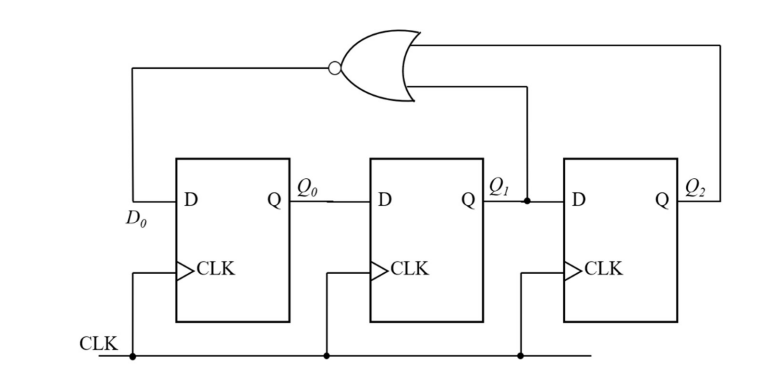
\includegraphics[scale = 0.8]{pics/1.png}
\end{figure}  
\end{center}

\subsection{Boolean Equation}
From the circuit diagram we can conclude:
\begin{align}
    D0 &=\overline{ (Q1 + Q2) }\\
    D1 &= Q0\\
    D2 &= Q1
\end{align}
\vspace{5pt}

\section{Truth Table}
\vspace{10pt}
\begin{center}
  \begin{tabularx}{0.6\textwidth} { 
  | >{\centering\arraybackslash}X 
  | >{\centering\arraybackslash}X 
  | >{\centering\arraybackslash}X
  | >{\centering\arraybackslash}X 
  | >{\centering\arraybackslash}X 
  | >{\centering\arraybackslash}X 
  | >{\centering\arraybackslash}X 
  | >{\centering\arraybackslash}X 
  | >{\centering\arraybackslash}X 
  | >{\centering\arraybackslash}X | }
\hline
\textbf{Q2} & \textbf{Q1} & \textbf{Q0} & \textbf{D2} & \textbf{D1} & \textbf{D0} & \textbf{Q2'} & \textbf{Q1'} & \textbf{Q0'}\\
\hline
0 & 0 & 0 & 1 & 0 & 0 & 1 & 0 & 0 \\  
\hline
0 & 0 & 1 & 1 & 0 & 0 & 1 & 0 & 0 \\  
\hline
0 & 1 & 1 & 1 & 0 & 0 & 1 & 0 & 0 \\  
\hline
1 & 1 & 0 & 1 & 0 & 0 & 1 & 0 & 0 \\  
\hline
1 & 0 & 0 & 1 & 0 & 0 & 1 & 0 & 0 \\  
\hline
\end{tabularx} \\
\vspace{6pt}
\textit{Truth table for the given circuit} 
\end{center}

\section{Implementation}
\vspace{15pt}
\begin{enumerate}[label=\Roman*]

    \item Make the connections between the seven segment display and the 7447 IC as shown below. 
    \begin{table}[htbp]
      \centering
      \begin{tabular}{|>{\centering\arraybackslash}m{2cm}|*{7}{>{\centering\arraybackslash}m{1.5cm}|}}
        \hline
        7447 & $\overline{a}$ & $\overline{b}$ & $\overline{c}$ & $\overline{d}$ & $\overline{e}$ & $\overline{f}$ & $\overline{g}$ \\
        \hline
        Display & a & b & c & d & e & f & g \\
        \hline
      \end{tabular}
      \label{tab:sample}
    \end{table}

    \item Connect the Arduino, 7447 and the two 7474 ICs according to below table.
    \begin{table}[htbp]
      \centering
      \begin{tabular}{|c|c|c|c|c|c|c|c|c|c|c|c|c|}
        \hline
        \multirow{2}{*}{} & \multicolumn{3}{c|}{INPUT} & \multicolumn{3}{c|}{OUTPUT} & \multicolumn{2}{c|}{CLOCK} & \multicolumn{4}{c|}{5V}\\
        \cline{2-7}
         & Q0 & Q1 & Q2 & Q0' & Q1' & Q2' & \multicolumn{2}{c|}{} & \multicolumn{4}{c|}{} \\
        \hline        
        Arduino & D6 & D7 & D8 & D2 & D3 & D4 & \multicolumn{2}{c|}{D13} & \multicolumn{4}{c|}{}\\
        \hline
        7474 & 5 & 9 & {} & 2 & 12 & {} & CLK1 & CLK2 & 1 & 4 & 10 & 13\\
        \hline
        7474 & {} & {} & 5 & {} & {} & 2 & CLK1 & CLK2 & 1 & 4 & 10 & 13\\
        \hline
        7447 & \multicolumn{3}{c|}{} & 7 & 1 & 2 & & & \multicolumn{4}{c|}{16}\\
        \hline 
      \end{tabular}
      \label{tab:merge-cells}
    \end{table}

    \item Hence we have implemented the divide by 5 counter digital circuit. Execute the circuit using below code. \vspace{10pt} \\
    \begin{tabularx}{1\textwidth} { 
    | >{\centering\arraybackslash}X |}
    \hline
    https://github.com/shr-eyas/FWC/blob/main/Embedded\%20C/counter.c\\
    \hline
    \end{tabularx} \\
\end{enumerate}


\bibliographystyle{ieeetr}
\end{document}
